% Do NOT change this "Section" title
% and do NOT add more "Section" level titles.
\section{Implementation}\label{sec:implementation}
The implementation of the simulator for project Naiad was created with the four following pillars in mind and tested with AUnit to ensure that all parts works as intended.

\subsection{Overall design using the Model View ViewModel approach}

The overall design of the simulator was implemented following the MVVM standard. At the top of this design is the graphical interface for the user. The graphical interface in turn holds several view models, which it gets its data from and calls on for updates of underlying layers. Each view model containing its own logic separated to that of the model itself to perform simpler tasks that is just for representation. There are 7 view models that all work on different parts of the program such as one for graphical representation, one for the PID values, one for the PID errors and one for setting each type of parameter.

\begin{figure}[h]
    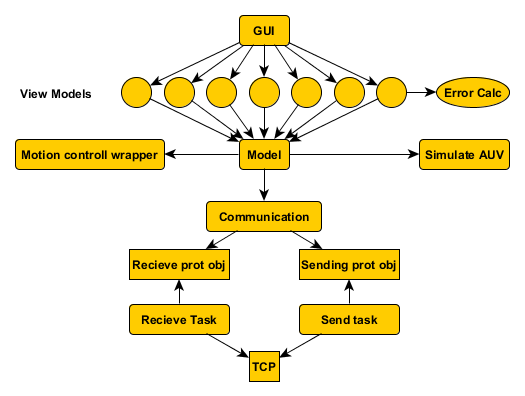
\includegraphics[width=0.5\textwidth]{./figure/Schedule.png}
    \caption{Simulator user interface}
    \label{fig:schedule}
\end{figure}


These view models then shares one common model that they are all keeping access to. This model in turns holds some simple logic together with the motion simulator part of the simulator and the different communication accesses, both with CAN over Ethernet and with a direct link to motion control. Where it with the update command fetches information of the simulated motion part and the communication part and sends it to the other respective part.

\begin{figure}[h]
    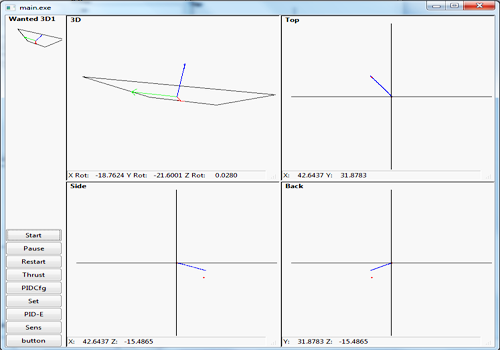
\includegraphics[width=0.5\textwidth]{./figure/Simulator-mod-500x350.png}
    \caption{Simulator user interface}
    \label{fig:one_column_figure}
\end{figure}
\pagebreak

\subsection{Usability and design in GTK ada}


The design of the user interface is built up as in figure \ref{fig:schedule} where the 3 views showing positioning in the 2 respective axis.

The interface is built up from using buttons where popup windows appear for setting data or monitoring actuators such as the motors without bloating the screen. To perform actions with a logic free interface the accessible view models are used to perform the various actions such as setting values, retrieving information, calling the periodic update for the simulated AUV and so on.

\subsection{Motion Simulation}
The implementation of the motion simulation is based on calculating the torque and the forces from the motors. These are then used together with the inertia, frictions, buoyancy and other aspects stored in the simulated motion to calculate the acceleration and angular acceleration that they would affect the AUV with on that specific time step.
 
The acceleration and angular acceleration is then used with numerical integration to receive the changes in velocity and angular velocity during that time frame, combining it with previous knowledge giving velocity and angular velocity. The velocity and angular velocity are then used in the same way and integrated into position and orientation. 

\subsection{Communication}

The design for the communication over TCP consists of two tasks and a interface that is used for communicating with those two tasks. The sender task retrieves data from a protected object, a set of information that could safely be used by different threads. From this protected object a sender task retrieves the data from the protected object that it is required to create the respective CAN messages to send.

On the other side of the communication package a receiver task reads the incoming CAN messages and writes the informative data into a receivers protected object which it is read when the simulator requests data from the communication section.

\subsection{Unit tests with AUnit}

For testing the sub parts of the system AUnit was used to test that each piece of logic was working as expected in order to fulfill the overall performance requirements of the system.  All the possible correct outcomes were to be predicted so that each sub system could be guaranteed to work properly. Though in the end as time was a key issue it was implemented on all key parts of the system which was easily accessible for testing and had a quite high risk of failure. Priorities to not test all part of the simulator was done where risks of failure was not high as the functionality was simple and could be tested lightly in other ways. This ended up saving key time while still getting the overall results that were wanted from the simulator in time.

